\documentclass{article}
	
\usepackage[margin=1in]{geometry}		% For setting margins
\usepackage{amsmath}				% For Math
\usepackage[]{amssymb}
\usepackage{amsmath}
\usepackage{gensymb}
\usepackage{fancyhdr}				% For fancy header/footer
\usepackage{graphicx}				% For including figure/image
\usepackage{cancel}					% To use the slash to cancel out stuff in work
\usepackage{wasysym}                % For cent symbol
\usepackage{needspace}              % To force item to next page

%%%%%%%%%%%%%%%%%%%%%%
% Set up fancy header/footer
\pagestyle{fancy}
\fancyhead[RO,R]{{\large\textbf{PHYS-102}}}
\fancyhead[LO,L]{\large{\textbf{Ch 17 Problem Set}}}
% \fancyhead[CO,C]{\large{\textbf{Part 1}}}
% \fancyhead[RO,R]{\today}
\fancyfoot[LO,L]{}
\fancyfoot[CO,C]{\thepage}
\fancyfoot[RO,R]{}
\renewcommand{\headrulewidth}{0.4pt}
\renewcommand{\footrulewidth}{0.4pt}
%%%%%%%%%%%%%%%%%%%%%%

\newcommand{\hmwkTitle}{Chapter 17 Temperature, Thermal Expansion, and Ideal Gas
Law}
% \newcommand{\hmwkDueDate}{February 12, 2014}
\newcommand{\hmwkClass}{PHYS-102}
% \newcommand{\hmwkClassTime}{}
% \newcommand{\hmwkClassInstructor}{Professor Isaac Newton}
\newcommand{\hmwkAuthorName}{\textbf{\underline{\hspace{3in}}}}

% math shortcuts
\newcommand\rr{\quad\Rightarrow\quad}

%
% Title Page
%

\title{
    \vspace{2in}
    \textmd{\textbf{\hmwkTitle}}\\
    \vspace{0.5in}
    \textmd{\textbf{\hmwkClass}}\\
    % \normalsize\vspace{0.1in}\small{Due\ on\ \hmwkDueDate\ at 3:10pm}\\
    % \vspace{0.1in}\large{\textit{\hmwkClassInstructor\ \hmwkClassTime}}
    \vspace{4in}
}

\author{\hmwkAuthorName}
\date{}
\begin{document}
\maketitle
\newpage
\begin{center}
    \section*{\textbf{\underline {Conceptual Questions}}}
\end{center}
\subsubsection*{
    1. Which has more atoms: 1 kg of iron or 1 kg of aluminum?
    See the Periodic Table or Appendix F. 
}
1 kg of aluminum will have more atoms. Aluminum has an atomic mass less than
iron. Since each Al atom is less massive than Fe atom, there will be more Al
atoms than Fe atoms in 1 kg.
\subsubsection*{
    10. Figure 17–18 shows a diagram of a simple \textbf{thermostat} used
    to control a furnace (or other heating or cooling system). The
    bimetallic strip consists of two strips of different metals bonded
    together. The electric switch (attached to the bimetallic strip) is
    a glass vessel containing liquid mercury that conducts electricity 
    when it can flow to touch both contact wires. Explain how this device
    controls the furnace and how it can be set at different temperatures
}
The bimetallic strip is made of two types of metal joined together. The metal of
the outside strip has a higher coefficient of linear expansion than that of the
inside strip, so it will expand and contract more dramatically. If
the temperature goes above the thermostat setting, the outer strip will expand
more than the inner, causing the spiral to wind more tightly and tilt the glass
vessel so that the liquid mercury flows away from the contact wires and the
heater turns off. If the temperature goes below the thermostat setting, the
vessel tilts back as the outer strip contracts more than the inner and the
spiral opens, and the heater turns on. Moving the temperature setting lever
changes the initial position of the glass vessel. For instance, if the lever is
set at 50, the vessel tilts with the mercury far from the contact wires. The
outer strip has to shrink significantly to uncurl the spiral enough to tilt the
vessel back.
\begin{figure}[h]
    \begin{center}
        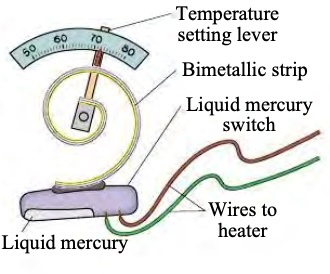
\includegraphics[width=0.4\textwidth]{figures/q10.jpg}
    \end{center}
\end{figure}
\subsubsection*{
    13. When a cold mercury-in-glass thermometer is first placed in a hot
    tub of water, the mercury initially descends a bit and then rises. Explain.
}
When the cold thermometer is placed in hot water, the glass part of the
thermometer will expand first, as heat is transferred to it first. This will
cause the mercury level in the thermomemeter to decrease. As heat is transferred
to the mercury inside the thermometer, the mercury will expand at a rate greater
than the glass, and the level of mercury in the thermometer will rise
\newpage
\begin{center}
    \section*{\textbf{\underline {Problems}}}
\end{center}
\begin{center}
    \subsection*{\textbf{\textit{17-1 Atomic Theory}}}
\end{center}
\subsubsection*{
    1. How does the number of atoms in a 21.5-g gold ring compare to
    the number in a silver ring of the same mass? 
}
\begin{align*}
    \intertext{The number of atoms in a pure substance can be found by dividing
    the mass of the substance by the mass of a single atom. Take the atomic masses
    of gold and silver  from the periodic table}
    \displaystyle\frac{N_{Au}}{N_{Ag}} &= \displaystyle\frac{\displaystyle\frac{2.15\times 10^{-2}kg}{(196.97\frac u {atom})(1.66\times 10^{-27}\frac{kg}{u})}}{\displaystyle\frac{2.15\times 10^{-2} kg}{(107.87\frac u{atom})(1.66\times 10^{-27}\frac{kg}{u})}} \\
    &= \displaystyle\frac{107.87\;atoms}{196.97\;atoms} \\
    &\approx 0.548 \\
    &\therefore \text{Au has about 55\% less
    atoms than Ag}
\end{align*}
\begin{center}
    \subsection*{\textbf{\textit{17-2 Temperature and Thermometers}}}
\end{center}
\subsubsection*{
    3. (a) “Room temperature” is often taken to be 68°F. What is this
    on the Celsius scale? (b) The temperature of the filament in a lightbulb
    is about 1900°C. What is this on the Fahrenheit scale?
}
\begin{align*}
    \intertext{a.}
    \frac 5 9 (68\degree F - 32) &= 20\degree C 
    \intertext{b.}
    \frac 9 5 (1900\degree C + 32) &= 3500\degree F
\end{align*}
\newpage
\begin{center}
    \subsection*{\textbf{\textit{17-4 Thermal Expansion}}}
\end{center}
\subsubsection*{
    7. The Eiffel Tower (Fig. 17–19) is built of wrought iron approximately 300 m
       tall. Estimate how much its height changes between January (average 
       temperature of 2°C) and July (average temperature of 25°C). Ignore the
       angles of the iron beams and treat the tower as a vertical beam
}
\begin{figure}[h]
    \begin{center}
        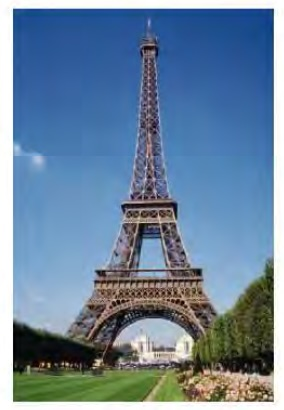
\includegraphics[width=0.2\textwidth]{figures/p7.jpg}
    \end{center}
\end{figure}
\begin{align*}
    \Delta l &= l_0 \alpha \Delta T \\
    \Delta l &= (300m)(12\times 10^{-6}C^{-1})(25\degree C - 2\degree C) \\
    \Delta l &= 0.08m
\end{align*}
\subsubsection*{
    8. A concrete highway is built of slabs 12 m long (15°C). How wide should
    the expansion cracks between the slabs be (at 15°C) to prevent buckling if
    the range of temperature is –30°C to ±50°C?
}
\begin{align*}
    \intertext{Note that if T = $-30\degree C$ like sometime during the winter,
    there is no longer any danger of buckling, so we disregard $-30\degree C$
    and focus on $50\degree C$}
    \Delta l &= l_0 \alpha \Delta T \\
    \Delta l &= (12m)(12\times 10^{-6}C^{-1})(50\degree C - 15\degree C) \\
    \Delta l &\approx 5.0\times 10^{-3}m
\end{align*}
\subsubsection*{
    17. It is observed that 55.50mL of water at 20°C completely fills a container
    to the brim. When the container and the water are heated to 60°C, 0.35 g of
    water is lost. (a) What is the coefficient of volume expansion of the container?
    (b) What is the most likely material of the container? Density of water at 60°C
    is 0.98324 g/mL.
}
\begin{align*}
    \intertext{Volume expansion is defined as $\Delta V = V_0 \beta \Delta T}
    \intertext{a.}
    V_{lost} &= (V_0+\Delta V)_{H_2O} - (V_0 + \Delta V)_{container} \\
    V_{lost} &= \Delta V_{H_2O} - \Delta V_{container} \\
    V_{lost} &= V_0 \beta_{H_2O} \Delta T - V_0 \beta_{container} \Delta T \\
    \beta_{container} &= \displaystyle\frac{V_0\beta_{H_2O}\Delta T}{V_0 \Delta
    T} - \displaystyle\frac{V_{lost}}{V_0\Delta T} \\
    \beta_{container} &= \beta_{H_20} -
    \displaystyle\frac{V_{lost}}{V_0\Delta T} \\
    \beta_{container} &= 210\times 10^{-6}C^{-1} -
    \displaystyle\frac{\frac{0.35g}{0.98324\frac g {mL}}}{(55.50mL)(60\degree C
    - 20\degree C)} \\
    \beta_{container} &\approx 5.0\times 10^{-5}C^{-1}
\end{align*}
\newpage
\begin{center}
    \subsection*{\textbf{\textit{17-7 and 17-8 Ideal Gas Law}}}
\end{center}
\subsubsection*{
    31. If 3.80 $m^3$ of a gas initially at STP is placed under a pressure of 3.20 atm,
    the temperature of the gas rises to 38.0°C. What is the volume?
}
\begin{align*}
    P_1V_1 = nRT_1 &\rr P_2V_2 = nRT_2  \\
    \displaystyle\frac{P_1V_1}{T_1} = nR &\rr \displaystyle\frac{P_2V_2}{T_2} =
    nR
    \intertext{Using the transitive property,}
    \displaystyle\frac{P_1V_1}{T_1} &= \displaystyle\frac{P_2V_2}{T_2}
    \intertext{Solving for $V_2$,}
    V_2 &= \displaystyle\frac{P_1V_1T_2}{P_2T_1} \\
    V_2 &= \displaystyle\frac{(1atm)(1.013\times 10^5 \frac N
    {m^2})(3.80m^3)(273K+38)}{(3.20atm)(1.013\times 10^5\frac N {m^2})(273K)} \\
        V_2 &\approx 1.35m^3
\end{align*}
\subsubsection*{
    34. If 14.00 mol of helium gas is at 10.0°C and a gauge pressure of 0.350 atm,
    calculate (a) the volume of the helium gas under these conditions, and (b) the
    temperature if the gas is compressed to precisely half the volume at a gauge
    pressure of 1.00 atm.
}
\begin{align*}
    \intertext{a. We use the Ideal Gas Law and solve for volume for find $V_1$}
    PV &= nRT \\ 
    V_1 &= \frac{nRT_1}{P_1} \\
    \intertext{Not that we need to use absolute pressure and not gauge pressure
    so 1 atm + our gauge pressure}
    V_1 &= \displaystyle\frac{(14.0mol)(8.314\frac J {mol\cdot
    K})(283K)}{1.350atm(1.013\times 10^5 \frac N {m^2})} \\
    V_1 &\approx 0.241 m^3 \\
    \intertext{b. We use the Ideal Gas Law and the transitive property to get an
    expression for $T_2$}
    nR = \displaystyle\frac{P_1V_1}{T_1} &\rr nR =
    \displaystyle\frac{P_2V_2}{T_2} \\
    T_2 &= T_1 \displaystyle\frac{P_2V_2}{P_1V_1} \\
    T_2 &= (283K)\left(\displaystyle\frac{(2atm)(\frac 1 2 \cdot
    0.241m^3)}{(1.350atm)(0.241m^3)}\right) \\
            T_2 &\approx 210K \approx -63\degree C
\end{align*}
\subsubsection*{
    37. A storage tank at STP contains 28.5 kg of nitrogen ($N_2$). (a) What is
    the volume of the tank? (b) What is the pressure if an additional 25.0 kg
    of nitrogen is added without changing the temperature?
}
\begin{align*}
    \intertext{a. Assume the nitrogen is an ideal gas. The number of moles of nitrogen is found from the atomic
    weight, and then the ideal gas law is used to calculate the volume of the gas.}
    n &= 28.5\;kg \left(\displaystyle\frac{1\;mol\;N_2}{28.01\times 10^{-3}kg}\right) \approx
    1017\;mol
    \intertext{Using Ideal Gas Law and solving for volume (note we are at STP),}
    V &= \displaystyle\frac{nRT}{P} \\
    V &= \displaystyle\frac{(1017mol)(8.314\frac J {mol\cdot
    K})(273K)}{1.013\times 10^5 \frac N {m^2}} \\
    V &\approx 22.8 m^3
    \intertext{b. T remains constant and we use the Ideal Gas Law and solve for
    pressure after finding the new mass in moles}
    n &= 53.5\;kg \left(\displaystyle\frac{1\;mol\;N_2}{28.01\times
    10^{-3}kg}\right)\approx1910\;mol \\
    P &= \displaystyle\frac{nRT}{V} \\
    P &= \displaystyle\frac{(1910mol)(8314\frac J {mol\cdot
    K})(273K)}{22.8m^3} \\
    P &\approx 1.9\times 10^5 \frac N {m^2} \approx 1.88\;atm
\end{align*}
\subsubsection*{
    41. A sealed metal container contains a gas at 20.0°C and 1.00 atm. To what
    temperature must the gas be heated for the pressure to double to 2.00 atm? 
    (Ignore expansion of the container.)
}
\begin{align*}
    \intertext{If there is no expansion of the container, that hints that volume
    is constant along with our moles and R constants.}
    \intertext{We can use the Ideal Gas Law and the transtive property to get
    an expression for final temperature $T_2$}
    \frac {nR}{V} = \frac {P_1}{T_1} &\rr \frac {nR}{V} = \frac {P_2}{T_2} \\
    \frac {P_1}{T_1} &= \frac {P_2}{T_2} \\
    T_2 &= T_1(\frac {P_2}{P_1}) \\
    T_2 &= (293K)(\frac {2atm}{1atm}) \\
    T_2 &= 586K\;or\;313\degree C
\end{align*}
\subsubsection*{
    44. A helium-filled balloon escapes a child’s hand at sea level and 20.0°C.
    When it reaches an altitude of 3600 m, where the temperature is 5.0°C and
    the pressure only 0.68 atm, how will its volume compare to that at sea level?
}
\begin{align*}
    \intertext{Ideal Gas Law and transitive property, then solve for the ratio
    of $\displaystyle\frac{V_2}{V_1}$}
    \displaystyle\frac{P_1V_1}{T_1} &= \displaystyle\frac{P_2V_2}{T_2} \\
    \displaystyle\frac{V_2}{V_1} &= \displaystyle\frac{P_1T_2}{P_2T_1} \\
    \displaystyle\frac{V_2}{V_1} &= \displaystyle\frac{(1atm)(278K)}{(0.68atm)(293K)} \approx 1.4 \\
                                 &\therefore\text{volume will increase by a factor of 1.4 times the original
    volume}
\end{align*}
\subsubsection*{
    50. An air bubble at the bottom of a lake 37.0 m deep has a volume of
    1.00 $cm^3$. If the temperature at the bottom is 5.5°C and at the top
    18.5°C, what is the volume of the bubble just before it reaches the surface?
}
\begin{align*}
    \intertext{We use the Ideal Gas Law and transitive property to get the
    expression for both locations (top and bottom)}
    \intertext{Let 1 = bot and 2 = top}
    \displaystyle\frac{P_1V_1}{T_1} &= \displaystyle\frac{P_2V_2}{T_2} \\
    \intertext{Solving for $V_2$}
    V_2 &= \displaystyle\frac{P_1V_1T_2}{T_1P_2} \\
    \intertext{Note that $P_1$ is atomsperic pressure above + $\rho gy$}
    V_2 &= \displaystyle\frac{(1atm+\rho gy)(V_1)(T_2)}{T_1P_2} \\
    V_2 &= \displaystyle\frac{[1.013\times 10^5 Pa +
        (1000\frac{kg}{m^3})(9.8\frac m {s^2})(37.0m)](1.0\times 10^{-6}m^3)(18\degree
C + 273K)}{(5.5\degree C + 273K)(1.013\times 10^5 Pa)} \\
        V_2 &\approx 4.79\times 10^{-6}m^3 \approx 4.79cm^3
\end{align*}
\begin{center}
    \subsection*{\textbf{\textit{17-9 Ideal Gas Law in Terms of Molecules;
    Avogadro's Number}}}
\end{center}
\subsubsection*{
    51. Calculate the number of $\frac{molecules}{m^3}$ in an ideal gas at STP.
}
\begin{align*}
    \intertext{At STP, 1 mole of ideal gas occupies 22.4 L.}
    \displaystyle\frac{1mol}{22.4L}\left(\displaystyle\frac{6.022\times
    10^{23}}{1mol}\right)\left(\displaystyle\frac{1L}{1.0\times 10^{-3}m^3}\right) \approx 2.69\times 10^{25}\;molecules/m^3
\end{align*}
\subsubsection*{
    52. How many moles of water are there in 1.000 L at STP? How many molecules?
}
\begin{align*}
    \intertext{We assume that the water is at 4$\degree$C so that its density is
    1000$\frac {kg}{m^3}$.}
    1.000L\left(\displaystyle\frac{1.0\times 10^{-3}m^3}{1.000L}\right)\left(\displaystyle\frac{1000kg}{1m^3}\right)\left(\displaystyle\frac{1mol}{(15.9994+2\times 1.00794)\times 10^{-3}kg}\right) &\approx 55.51mol \\
    55.51mol\left(\displaystyle\frac{6.022\times 10^{23}\;molecules}{1mol}\right) &\approx 3.343\times 10^{25}\;molecules
\end{align*}
\newpage
\begin{center}
    \subsection*{\textbf{\textit{General Problems}}}
\end{center}
\subsubsection*{
    69. A house has a volume of $870\;m^3$. (a) What is the total mass of air inside
    the house at 15°C? (b) If the temperature drops to –15°C, what mass of air
    enters or leaves the house?
}
\begin{align*}
    \intertext{To do this problem, the “molecular weight” of air is needed. If we approximate air as 70\% $N_2$ (molecular weight 28) and 30\% $O_2$ (molecular weight 32), 
    then the average molecular weight is $0.70(28)+0.30(32)= 29.2$.}
    \intertext{a. Treat the air as an ideal gas. Assume that the pressure is 1.00 atm.}
    PV &= nRT \\
    n &= \displaystyle\frac{PV}{RT} \\
    n &= \displaystyle\frac{(1.013\times 10^5 \frac N {m^2})(870m^3)}{(8.314\frac J {mol\cdot})(293K)} \\
    n &\approx 3.6178\times 10^4\;moles \\
    m &= (3.6178\times 10^4\;moles )(29.2\times 10^{-3}kg/mol) = 1056.4kg
    \approx 1100kg
    \intertext{b. Find the mass of air at the lower temperature, and then subtract the mass at the higher temperature.}
    n &= \displaystyle\frac{PV}{RT} \\
    n &= \displaystyle\frac{(1.013\times 10^5 \frac N {m^2})(870m^3)}{(8.314\frac J {mol\cdot K})(263K)} \\
    n &= 4.0305\times 10^4\;moles \\
    m &= (4.0305\times 10^4\;moles )(29.2\times 10^{-3}kg/mol) = 1176.9kg \\
    \intertext{\therefore\text{The mass entering the house is 1176.9 kg − 1056.4 kg = 120.5 kg $\approx$ 100 kg.}}
\end{align*}
\end{document}
